\documentclass[a4paper]{tufte-handout}

\usepackage[utf8]{inputenc}
\usepackage[english]{babel}
\usepackage{mathtools}
\usepackage{amsthm}
\usepackage{tkz-graph}
\usepackage{booktabs}
\usepackage{enumitem}
\usepackage[caption=false]{subfig}
\usetikzlibrary{arrows.meta}

%% Setting the headings to bold instead of italic
%\titleformat{\chapter}%
%[display]% shape
%{\relax\ifthenelse{\NOT\boolean{@tufte@symmetric}}{\begin{fullwidth}}{}}% format applied to label+text
%	{\bfseries\huge\thechapter}% label
%	{0pt}% horizontal separation between label and title body
%	{\huge\rmfamily\bfseries}% before the title body
%	[\ifthenelse{\NOT\boolean{@tufte@symmetric}}{\end{fullwidth}}{}]% after the title body
%
%\titleformat{\section}%
%[hang]% shape
%{\normalfont\large\smallcaps}% format applied to label+text
%{\thesection}% label
%{1em}% horizontal separation between label and title body
%{}% before the title body
%[]% after the title body

%\titleformat{\subsection}%
%[hang]% shape
%{\normalfont\large\bfseries}% format applied to label+text
%{\thesubsection}% label
%{1em}% horizontal separation between label and title body
%{}% before the title body
%[]% after the title body
%
%\titleformat{\paragraph}%
%[runin]% shape
%{\normalfont\bfseries}% format applied to label+text
%{\theparagraph}% label
%{1em}% horizontal separation between label and title body
%{}% before the title body
%[]% after the title body


%% improving tuftebreak
%% http://tex.stackexchange.com/questions/291746/tufte-latex-newthought-after-section
\makeatletter
\def\tuftebreak{%
	\if@nobreak\else
	\par
	\ifdim\lastskip<\tufteskipamount
	\removelastskip \penalty -100
	\tufteskip
	\fi
	\fi
}
\makeatother

%% Change the spacing in the itemize environment
\setlist[itemize]{nosep}

%% Defining the theorem environments
\newtheorem*{theorem}{Theorem}
\theoremstyle{definition}
\newtheorem*{definition}{Definition}
\theoremstyle{remark}
\newtheorem*{remark}{Remark}

%% Defining my colors
\definecolor{myBlue}{HTML}{809BC8}
\definecolor{myGreen}{HTML}{64C204}
\definecolor{myRed}{HTML}{FF6666}

\title{Congestion Games with Malicious Players}
\author{Daniel Alexander Mock}
\date{\today}

\begin{document}
	\maketitle
	
	\begin{abstract}
		We introduce the notion of a \emph{malicious player} whose objective is to maximize the cost of the rational players.
	\end{abstract}

\section{Introduction}

\newthought{Game theory} studies mathematical models of interactions between self-interested, rational agents. 
It has many applications in computer science, operations research, economics, social science and even in biology. 
A \emph{game} has players, a set of feasible strategies for every player and 

\section{Defining the congestion game}
\newcommand{\tupel}[1]{\left(#1\right)}
\newthought{In this section} we introduce the concept of \emph{congestion games} as preliminaries for the rest of the paper.
Every congestion game is based on a flow network $G$ with a source $s$ and a sink $d$ where the agents control a flow $f$ from $s$ to $t$.
Every agent chooses a path from the source to the sink, with the aim to minimize the occurring delay on the path.
The delay is the sumTODO

\begin{definition}[Congestion game]
	We define a \emph{symmetrical\footnote{symmetric: every agent has the same utility function}, non-atomic\footnote{non-atomic: the players are not discrete entities, but they are a continuum. But do not worry, this detail will be sufficiently explained later.}, congestion game} $\mathcal G$ as a tuple $(G, \vec{\ell}, v)$ where
	\begin{itemize}
		\item $G = (E, V)$ is a flow network, where $E$ is the edge set, $V$ the vertex set, $s$ the source and $t$ the drain,
		\item $\vec{\ell}$ is vector consisting of latency functions for every edge in $E$,
		\item and $v$ is the desired (real) flow value.
	\end{itemize}
	Additionally, we define $\Pi$ as the set of all $s-t$ paths in $G$.
\end{definition}

\begin{remark}
	We only consider latency functions $\ell \colon \mathbb R_+ \to \mathbb R_+$ which are nondecreasing.
\end{remark} 

BSP
\begin{definition}[Flow]
	A \emph{flow} in a flow network is a function $f \colon \Pi \to \mathbb R_+$ which maps every $s-t$ path to a flow value.
	The \emph{value} of a flow is $|f| = \sum_{P \in \Pi} f(P)$ the sum of the flow values of every path in the network.
	We denote the set of flows in $\mathcal G$ with flow value $v$ as $F(\mathcal G, v)$.
		\marginnote{The abuse of notation indicates that our definition of a flow is equivalent to the usual one given by defining it as a function $f \colon E \to \mathbb R_+$ with flow conservation and symmetry but without the capacity constraint. }
	The \emph{load} on an edge $e \in E$ is $f(e) = \sum_{P \in \Pi \colon e \in P} f(P)$ the summed up flow value of the paths which contain $e$.
\end{definition}



	\marginnote{As an attentive reader you certainly noticed that this game degenerates to a min-cost flow problem if the latency functions are constants.}

\section{Introducing the malicious player}

\section{Lower bounds on the price of malice}

\newthought{How high} can the price of malice be?
In this section we study the havoc a malicious player is able to cause by constructing an example network.
Though a strict upper bound for the price of malice is not yet known.
Which properties of a network may cause a high price of malice?
We take a look at this two main reasons:
\begin{enumerate}
	\item edges that \emph{congest fast} if a small load is added by a malicious player
	\item and \emph{long paths} that a malicious player can choose to increase the load of as many edges as possible.
\end{enumerate}

\section{Windfall of malice}

In the previous section we experienced the havoc a malicious player is capable of causing in a congestion game.
But is the opposite possible -- that there is an improvement by the malicious player?
After all, there are many paradoxes of this kind in game theory.
In this section we will see that there is indeed a \emph{Windfall of Malice}, but first we will take a look at \emph{Breass' paradox} to construct, and understand the nature of, that paradox.

\subsection{Braess' paradox}

Braess' paradox was discovered by Dietrich Braess in 1968 and demonstrates how an additional strategic option is able to cause a worse stable solution in a congestion game than before.
In Figure \ref{braess-base} we see a congestion game.
Because of its symmetry, the Nashflow is divided in two equal parts -- on the upper path flows 1/2 and on the lower one, too.
The resulting Nashdelay is thus 1.25.
In the real world, we could interpret this game as a street network where daily people commute from $s$ to $t$ and the nashdelay is the length of a traffic jam.

If the city council however decides to add an additional road between $p$ and $q$ (see \ref{braess-complete}) to decrease the congestion, they achieve the opposite -- the nashdelay increases because nash flow only uses the path $s-p-q-t$.
But why?
Because the delay of the upper and of the lower path are always bigger than the delay of the central path:
Let $P$ be the upper path $s-p-t$ and $P^*$ the central path $s-p-q-t$.
Because the flow value is $v=1$ the load of an edge cannot exceed 1.
\begin{align*}
	L(P) = f(e_1)/2 + 1 \geq f(e_1)/2 + f(e_2)/2 + f(e_3)/2 = L(P^*) 
\end{align*}
By symmetry this also holds for the lower path.
And because the old nash flow is not stable anymore, the only nash flow is that one which concentrates all on $P^*$.
But the nash delay is here $L(P^*) = 1.5$.

\begin{figure}
	\subfloat[Congestion game with flow value $v=1$\label{braess-base}]{
		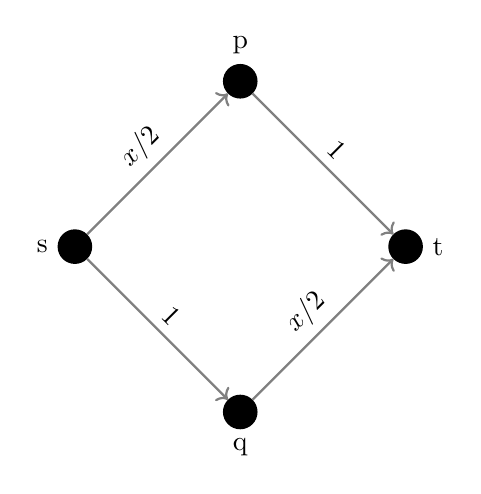
\begin{tikzpicture}[scale=0.7]
			\SetGraphUnit{2}
			\GraphInit[vstyle=Classic]
			\SetUpEdge[style={->, thick}, color=gray]
			\tikzset{LabelStyle/.style = {fill=none, sloped, above}}
			
			% Knoten
			\Vertices[unit=3]{circle}{t,p,s,q}
			
			% Kanten
			\Edge[label=$x/2$](s)(p)
			\Edge[label=$x/2$](q)(t)
			\Edge[label=$1$](s)(q)
			\Edge[label=$1$](p)(t)
		\end{tikzpicture} 
	}
	\subfloat[adding the shortcut\label{braess-complete}]{
		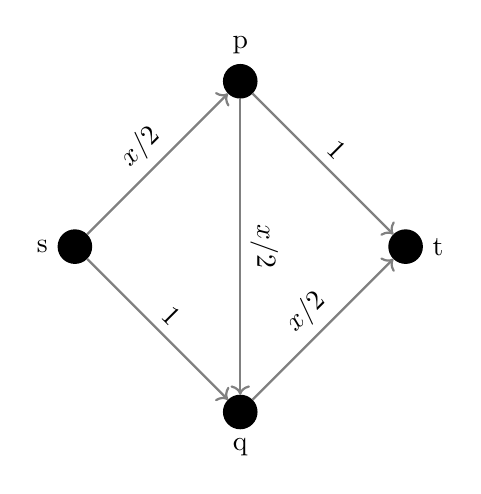
\begin{tikzpicture}[scale=0.7]
			\SetGraphUnit{2}
			\GraphInit[vstyle=Classic]
			\SetUpEdge[style={->, thick}, color=gray]
			\tikzset{LabelStyle/.style = {fill=none, sloped, above}}
			
			% Knoten
			\Vertices[unit=3]{circle}{t,p,s,q}
			
			% Kanten
			\Edge[label=$x/2$](s)(p)
			\Edge[label=$x/2$](q)(t)
			\Edge[label=$1$](s)(q)
			\Edge[label=$1$](p)(t)
			% Abkürzung
			\Edge[label=$x/2$](p)(q)
		\end{tikzpicture}
	}
	\caption{Example network for Braess' paradox, first without, then with the shortcut. The Nashdelay increases form 1.25 to 1.5.}
\end{figure}

But before we are able to proceed to the windfall of malice we have to make a small adjustment of the congestion game above.
We replace the edge $p-q$ with a slightly more complex subgraph (see \ref{braess-modified}). 
But this subgraph behaves exactly like the edge:
Let there be a nash flow with flow value $u$ between $p$ and $q$.
Then it is divided equally between the path $p-m-q$ and $p-n-q$ and thus has a nash delay of $u/2$ -- exactly like a nash flow between $p$ and $q$ in the old network.
\begin{marginfigure}
	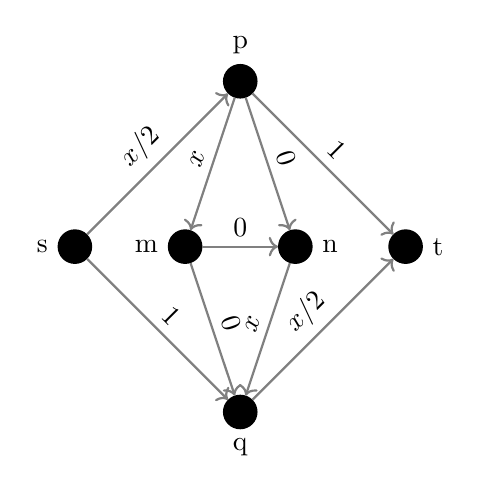
\begin{tikzpicture}[scale=0.7]
	\SetGraphUnit{2}
		\GraphInit[vstyle=Classic]
		\SetUpEdge[style={->, thick}, color=gray]
		\tikzset{LabelStyle/.style = {fill=none, sloped, above}}
		
		% Knoten
		\Vertices[unit=3]{circle}{t,p,s,q}
		
		% Kanten
		\Edge[label=$x/2$](s)(p)
		\Edge[label=$x/2$](q)(t)
		\Edge[label=$1$](s)(q)
		\Edge[label=$1$](p)(t)
		
		%innen
		\EA[Lpos=180](s){m}
		\EA[unit=2](m){n}
		\Edge[label=$0$](p)(n)
		\Edge[label=$0$](m)(n)
		\Edge[label=$0$](m)(q)
		\Edge[label=$x$](p)(m)
		\Edge[label=$x$](n)(q)
	\end{tikzpicture}
	\caption{Modified network which has also a nash delay of 1.5}
	\label{braess-modified}
\end{marginfigure}


\subsection{Reverting Braess' paradox with the malicious player}

After discussing Braess' paradox we address the windfall of malice.
What happens if we add a malicious player to the game above?
We see a \emph{decrease} of the nash delay!
In some manner, the windfall of malice counteracts Braess' paradox.

To analysis this behaviour, we first determine the malicious best response.
The \textsc{Mbr} is always the path $s,p,m,n,q,t$ because this covers all edges with non-constant latency functions (similar like in the section before).
\begin{figure}
	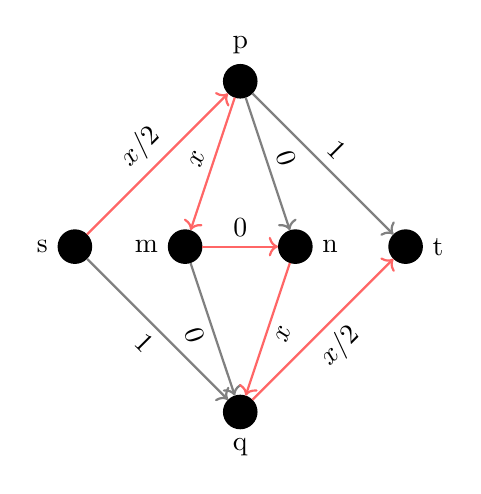
\begin{tikzpicture}[scale=0.7]
	\SetGraphUnit{2}
	\GraphInit[vstyle=Classic]
	\SetUpEdge[style={->, thick}, color=gray]
	\tikzset{LabelStyle/.style = {fill=none, sloped, above}}
	
	% Knoten
	\Vertices[unit=3]{circle}{t,p,s,q}
	\EA[Lpos=180](s){m}
	\EA[unit=2](m){n}
	
	% Kanten
	\Edge[label=$1$](p)(t)
	\Edge[label=$0$](p)(n)
	\SetUpEdge[style={->, thick}, color=myRed]
	\tikzset{LabelStyle/.style = {fill=none, sloped, above}}
	\Edge[label=$x/2$](s)(p)
	\Edge[label=$x$](p)(m)
	\Edge[label=$0$](m)(n)
	
	\SetUpEdge[style={->, thick}, color=gray]
	\tikzset{LabelStyle/.style = {fill=none, sloped, below}}
	\Edge[label=$1$](s)(q)
	\Edge[label=$0$](m)(q)
	\SetUpEdge[style={->, thick}, color=myRed]
	\tikzset{LabelStyle/.style = {fill=none, sloped, below}}
	\Edge[label=$x$](n)(q)
	\Edge[label=$x/2$](q)(t)
	
	
	\end{tikzpicture}
	\caption{Game with a malicious player's \textsc{Mbr} drawn in with red colour.}
	\label{wof-mbr}
\end{figure} 


\end{document}
